%!TEX root =../../../course-notes.tex
% ^ leave for LaTeXTools build functionality


\begin{observation}
Several properties of the real numbers, such as commutivity:
\[
  x + y = y + x
\]
also hold for Euclidean vectors with multiple components:
\[
\begin{bmatrix}x_1\\x_2\end{bmatrix}
+
\begin{bmatrix}y_1\\y_2\end{bmatrix}
=
\begin{bmatrix}y_1\\y_2\end{bmatrix}
+
\begin{bmatrix}x_1\\x_2\end{bmatrix}
\]
\end{observation}

\begin{activity}{20}\smallSlideText
Consider each of the following properties of the real numbers
\(\IR^1\). Label each property as \textbf{valid} if the property also
holds for two-dimensional Euclidean vectors 
\(\vec u,\vec v,\vec w\in\IR^2\) and scalars \(a,b\in\IR\),
and \textbf{invalid} if it does not.
\begin{multicols}{2}
\begin{enumerate}
  \item \(\vec u+(\vec v+\vec w)=
        (\vec u+\vec v)+\vec w\).
  \item \(\vec u+\vec v=
        \vec v+\vec u\).
  \item There exists some \(\vec z\)
        where \(\vec v+\vec z=\vec v\).
  \item There exists some \(-\vec v\)
        where \(\vec v+(-\vec v)=\vec z\).
  \item If \(\vec u\not=\vec v\), then \(\frac{1}{2}(\vec u+\vec v)\)
        is the only vector equally distant from both \(\vec u\) and \(\vec v\)
  \item \(a(b\vec v)=(ab)\vec v\).
  \item \(1\vec v=\vec v\).
  \item If \(\vec u\not=\vec 0\), then there exists some scalar \(c\) 
        such that \(c\vec u=\vec v\).
  \item \(a(\vec u+\vec v)=a\vec u+a\vec v\).
  \item \((a+b)\vec v=a\vec v+b\vec v\).
\end{enumerate}
\end{multicols}
\end{activity}

\begin{definition}
  A \term{vector space} \(V\) is any collection of mathematical objects with
  associated addition \(\oplus\) and scalar multiplication \(\odot\)
  operations that satisfy the following properties. 
  Let \(\vec u,\vec v,\vec w\) belong to \(V\), and let \(a,b\) be scalar numbers.

  \vectorSpaceProperties
\end{definition}

\begin{observation}

  Every \term{Euclidean vector space}
  \[
    \IR^n=\setBuilder{\begin{bmatrix}x_1\\x_2\\\vdots\\x_n\end{bmatrix}}{x_1,x_2,\dots,x_n\in\IR}
  \] 
  satisfies all eight requirements for the usual definitions of addition
  and scalar multiplication,
  but we will also study other types of vector spaces.
\end{observation}

\begin{observation}
The space of \(m \times n\)\term{matrices}
  \[
    M_{m,n}=\setBuilder{\begin{bmatrix}a_{11}  & a_{12} & \cdots & a_{1n} \\ a_{21} & a_{22} & \cdots & a_{2n} \\\vdots & \vdots & & \ddots & \vdots \\a_{m1} & a_{m2} & \cdots & a_{mn} \end{bmatrix}}{a_{11},\ldots,a_{mn} \in\IR}
  \] 
  satisfies all eight requirements for component-wise addition
  and scalar multiplication.
\end{observation}



\begin{remark}
  Every Euclidean space \(\IR^n\) is a vector space, but there are other
  examples of vector spaces as well. 

  \vspace{1em}
  
  For example, consider the
  set \(\IC\) of complex numbers with the usual defintions of
  addition and scalar multiplication, and let 
  \(\vec u=a+b\mathbf{i}\), \(\vec v=c+d\mathbf{i}\), and \(\vec w=e+f\mathbf{i}\). Then

  \begin{align*}
    \vec u+(\vec v+\vec w)
      &=
    (a+b\mathbf{i})+((c+d\mathbf{i})+(e+f\mathbf{i}))
      \\&=
    (a+b\mathbf{i})+((c+e)+(d+f)\mathbf{i})
	\\&=(a+c+e)+(b+d+f)\mathbf{i}
    \\&=((a+c)+(b+d)\mathbf{i})+(e+f\mathbf{i})
      \\&=
    (\vec u+\vec v)+\vec w
  \end{align*}

  All eight properties can be verified in this way.
\end{remark}

\begin{remark}
  The following sets are just a few examples of vector spaces, with the usual/natural
  operations for addition and scalar multiplication.
  \begin{itemize}
    \item \(\IR^n\): Euclidean vectors with \(n\) components.
    \item \(\IC\): Complex numbers.
    \item \(M_{m,n}\): Matrices of real numbers with \(m\) rows and
          \(n\) columns.
    \item \(\P^n\): Polynomials of degree \(n\) or less.
    \item \(\P\): Polynomials of any degree.
    \item \(C(\IR)\): Real-valued continuous functions.
  \end{itemize}
\end{remark}

\begin{remark}
  Previously, we defined a \term{vector space} \(V\) to be any collection of
  mathematical objects with
  associated addition and scalar multiplication operations that satisfy
  the following eight properties for all \(\vec u,\vec v,\vec w\) in \(V\),
  and all scalars (i.e. real numbers) \(a,b\).

  \vectorSpaceProperties
\end{remark}

\begin{activity}{20}
  Consider the set \(V=\setBuilder{(x,y)}{y=e^x}\) with operations defined by
  \[
    (x_1,y_1)\oplus (x_2,y_2)=(x_1+x_2,y_1y_2)
      \hspace{3em}
    c\odot (x_1,y_1)=(cx_1,y_1^c)
  \]
  \begin{subactivity}
  Show that \(V\) satisfies the distributive property
  \[(a+b)\odot (x_1,y_1)=\left(a\odot (x_1,y_1)\right)\oplus \left(b\odot (x_1,y_1)\right)\]
  by simplifying both sides and verifying they are the same
  expression.
  \end{subactivity}
  \begin{subactivity}%optional
  Show that \(V\) contains an additive identity element satisfying
  \[(x_1,y_1)\oplus\vec{z}=(x_1,y_1)\]
  for all \((x_1,y_1)\in V\)
  by choosing appropriate values for \(\vec{z}=(\unknown,\unknown)\). 
  \end{subactivity}
\end{activity}


\begin{remark}
  It turns out \(V=\setBuilder{(x,y)}{y=e^x}\) with operations defined by
  \[
    (x_1,y_1)\oplus (x_2,y_2)=(x_1+x_2,y_1y_2)
      \hspace{3em}
    c\odot (x_1,y_1)=(cx_1,y_1^c)
  \]
  satisifes all eight properties.

  \vectorSpaceProperties

  Thus, \(V\) is a vector space.
\end{remark}





\begin{activity}{15}
  Let \(V=\setBuilder{(x,y)}{x,y\in\IR}\) have operations defined by
  \[
    (x_1,y_1)\oplus (x_2,y_2)=(x_1+y_1+x_2+y_2,x_1^2+x_2^2)
      \hspace{3em}
    c\odot (x_1,y_1)=(x_1^c,y_1+c-1)
  .\]

  \begin{subactivity}
    Show that \(1\) is the scalar multiplication identity element
	by simplifying \(1\odot(x,y)\) to \((x,y)\).
  \end{subactivity}

  \begin{subactivity}
    Show that \(V\) does not have an additive identity element by showing that 
	\((0,-1)\oplus\vec z\not=(0,-1)\) no matter how
    \(\vec z=(z,w)\) is chosen.
  \end{subactivity}

  \begin{subactivity}
    Is \(V\) a vector space?
  \end{subactivity}
\end{activity}

\begin{activity}{15}
  Let \(V=\setBuilder{(x,y)}{x,y\in\IR}\) have operations defined by
  \[
    (x_1,y_1)\oplus (x_2,y_2)=(x_1+x_2,y_1+3y_2)
      \hspace{3em}
    c\odot (x_1,y_1)=(cx_1,cy_1)
  .\]

  \begin{subactivity}
    Show that scalar multiplication distributes over vector addition, i.e.
	\[ c \odot \left( (x_1,y_1) \oplus (x_2,y_2) \right) = c\odot (x_1,y_1) \oplus c\odot (x_2,y_2)\]
	for \textbf{all} \(c\in \IR,\, (x_1,y_1),(x_2,y_2) \in V\). 
\end{subactivity}

  \begin{subactivity}
    Show that vector addition is not associative, i.e. 
  \[ (x_1,y_1) \oplus \left((x_2,y_2) \oplus (x_3,y_3)\right) \neq \left((x_1,y_1)\oplus (x_2,y_2)\right) \oplus (x_3,y_3)\]
  for \textbf{some} vectors \( (x_1,y_1), (x_2,y_2), (x_3,y_3) \in V\).
  \end{subactivity}

  \begin{subactivity}
    Is \(V\) a vector space?
  \end{subactivity}
\end{activity}


\begin{definition}
  A \term{linear combination} of a set of vectors
  \(\{\vec v_1,\vec v_2,\dots,\vec v_m\}\) is given by
  \(c_1\vec v_1+c_2\vec v_2+\dots+c_m\vec v_m\) for any choice of
  scalar multiples \(c_1,c_2,\dots,c_m\).

	\vspace{2em}

  For example, we can say \(\begin{bmatrix}3 \\0 \\ 5\end{bmatrix}\) 
  is a linear combination of the vectors \(\begin{bmatrix} 1 \\ -1 \\ 2 \end{bmatrix}\) 
  and \(\begin{bmatrix} 1 \\ 2 \\ 1 \end{bmatrix}\) since 
  \[
    \begin{bmatrix} 3 \\ 0 \\ 5 \end{bmatrix} = 
    2 \begin{bmatrix} 1 \\ -1 \\ 2 \end{bmatrix} + 
    1\begin{bmatrix} 1 \\ 2 \\ 1 \end{bmatrix}
  \]
\end{definition}

\begin{definition}
  The \term{span} of a set of vectors is the collection of all linear
  combinations of that set:
  \[
    \vspan\{\vec v_1,\vec v_2,\dots,\vec v_m\} =
    \setBuilder{c_1\vec v_1+c_2\vec v_2+\dots+c_m\vec v_m}{
    c_i\in\IR}.
  \]

	\vspace{2em}

  For example:

  \[
    \vspan\setList
    {
      \begin{bmatrix} 1 \\ -1 \\ 2 \end{bmatrix},
      \begin{bmatrix} 1 \\ 2 \\ 1 \end{bmatrix}
    } = \setBuilder
    {
      a\begin{bmatrix} 1 \\ -1 \\ 2 \end{bmatrix}+
      b\begin{bmatrix} 1 \\ 2 \\ 1 \end{bmatrix}
    }{
      a,b\in\IR
    }
  \]
\end{definition}

\begin{activity}{10}
  Consider \(\vspan\left\{\begin{bmatrix}1\\2\end{bmatrix}\right\}\).
  \begin{subactivity}
    Sketch

    \(1\begin{bmatrix}1\\2\end{bmatrix}=\begin{bmatrix}1\\2\end{bmatrix}\),
    \hfill\(3\begin{bmatrix}1\\2\end{bmatrix}=\begin{bmatrix}3\\6\end{bmatrix}\),
    \hfill\(0\begin{bmatrix}1\\2\end{bmatrix}=\begin{bmatrix}0\\0\end{bmatrix}\),
    \hfill and \(-2\begin{bmatrix}1\\2\end{bmatrix}=\begin{bmatrix}-2\\-4\end{bmatrix}\) 

    in the \(xy\) plane.
  \end{subactivity}
  \begin{subactivity}
    Sketch a representation of all the vectors belonging to
    \(
      \vspan\setList{\begin{bmatrix}1\\2\end{bmatrix}}
        =
      \setBuilder{a\begin{bmatrix}1\\2\end{bmatrix}}{a\in\IR}
    \)
    in the \(xy\) plane.
  \end{subactivity}
\end{activity}





\begin{activity}{10}
  Consider \(\vspan\left\{\begin{bmatrix}1\\2\end{bmatrix},
  \begin{bmatrix}-1\\1\end{bmatrix}\right\}\).
  \begin{subactivity}
    Sketch the following linear combinations in the \(xy\) plane.
    \[
    1\begin{bmatrix}1\\2\end{bmatrix}+
    0\begin{bmatrix}-1\\1\end{bmatrix}\hspace{3em}
    0\begin{bmatrix}1\\2\end{bmatrix}+
    1\begin{bmatrix}-1\\1\end{bmatrix}\hspace{3em}
    1\begin{bmatrix}1\\2\end{bmatrix}+
    1\begin{bmatrix}-1\\1\end{bmatrix}
    \]
    \[
    -2\begin{bmatrix}1\\2\end{bmatrix}+
    1\begin{bmatrix}-1\\1\end{bmatrix}\hspace{3em}
    -1\begin{bmatrix}1\\2\end{bmatrix}+
    -2\begin{bmatrix}-1\\1\end{bmatrix}
    \]
  \end{subactivity}
  \begin{subactivity}
    Sketch a representation of all the vectors belonging to
    \(\vspan\left\{\begin{bmatrix}1\\2\end{bmatrix},
     \begin{bmatrix}-1\\1\end{bmatrix}\right\}\)
    in the \(xy\) plane.
  \end{subactivity}
\end{activity}

\begin{activity}{5}
    Sketch a representation of all the vectors belonging to
    \(\vspan\left\{\begin{bmatrix}6\\-4\end{bmatrix},
     \begin{bmatrix}-3\\2\end{bmatrix}\right\}\)
    in the \(xy\) plane.
\end{activity}

\begin{remark}
	Recall these definitions from last class:
\begin{itemize}
	\item
  A \term{linear combination} of vectors is given by adding scalar
  multiples of those vectors, such as:
  \[
    \begin{bmatrix} 3 \\ 0 \\ 5 \end{bmatrix} =
    2 \begin{bmatrix} 1 \\ -1 \\ 2 \end{bmatrix} +
    1\begin{bmatrix} 1 \\ 2 \\ 1 \end{bmatrix}
  \]

\item The \term{span} of a set of vectors is the collection of all linear
  combinations of that set, such as:
  \[
    \vspan\setList
    {
      \begin{bmatrix} 1 \\ -1 \\ 2 \end{bmatrix},
      \begin{bmatrix} 1 \\ 2 \\ 1 \end{bmatrix}
    } = \setBuilder
    {
      a\begin{bmatrix} 1 \\ -1 \\ 2 \end{bmatrix}+
      b\begin{bmatrix} 1 \\ 2 \\ 1 \end{bmatrix}
    }{
      a,b\in\IR
    }
  \]
 \end{itemize}
\end{remark}


\begin{activity}{15}
  The vector
  \(\begin{bmatrix}-1\\-6\\1\end{bmatrix}\) belongs to
  \(\vspan\left\{\begin{bmatrix}1\\0\\-3\end{bmatrix},
  \begin{bmatrix}-1\\-3\\2\end{bmatrix}\right\}\) exactly when
  there exists a solution to the vector equation
  \(x_1\begin{bmatrix}1\\0\\-3\end{bmatrix}+
  x_2\begin{bmatrix}-1\\-3\\2\end{bmatrix}
  =\begin{bmatrix}-1\\-6\\1\end{bmatrix}\).

  \begin{subactivity}
    Reinterpret this vector equation as a system of linear equations.
  \end{subactivity}

  \begin{subactivity}
    Find its solution set, using technology to find \(\RREF\) of its
    corresponding augmented matrix.
  \end{subactivity}

  \begin{subactivity}
    Given this solution set, does
    \(\begin{bmatrix}-1\\-6\\1\end{bmatrix}\) belong to
    \(\vspan\left\{\begin{bmatrix}1\\0\\-3\end{bmatrix},
    \begin{bmatrix}-1\\-3\\2\end{bmatrix}\right\}\)?
  \end{subactivity}
\end{activity}

\begin{fact}
  A vector \(\vec b\) belongs to
  \(\vspan\{\vec v_1,\dots,\vec v_n\}\) if and only if
	the vector equation \(x_1 \vec{v}_1+\cdots+x_n \vec{v_n}=\vec{b}\) is consistent.
\end{fact}

\begin{quickcheck}
The following are all equivalent statements:
\begin{itemize}
\item The vector \(\vec{b}\) belongs to \(\vspan\{\vec v_1,\dots,\vec v_n\}\).
\item The vector equation \(x_1 \vec{v}_1+\cdots+x_n \vec{v_n}=\vec{b}\) is consistent.
\item The linear system corresponding to
  \([\vec v_1\,\dots\,\vec v_n \,|\, \vec b]\)
  is consistent.
\item  \(\RREF[\vec v_1\,\dots\,\vec v_n \,|\, \vec b]\)
  doesn't have a row \([0\,\cdots\,0\,|\,1]\)
  representing the contradiction \(0=1\).
\end{itemize}
\end{quickcheck}

\begin{activity}{10}
  Determine if
  \(\begin{bmatrix}3\\-2\\1 \\ 5\end{bmatrix}\) belongs to
  \(\vspan\left\{\begin{bmatrix}1\\0\\-3 \\ 2\end{bmatrix},
  \begin{bmatrix}-1\\-3\\2 \\ 2\end{bmatrix}\right\}\)
  by solving an appropriate vector equation.
\end{activity}





\begin{activity}{5}
  Determine if
  \(\begin{bmatrix}-1\\-9\\0\end{bmatrix}\) belongs to
  \(\vspan\left\{\begin{bmatrix}1\\0\\-3\end{bmatrix},
  \begin{bmatrix}-1\\-3\\2\end{bmatrix}\right\}\)
  by solving an appropriate vector equation.
\end{activity}


\begin{activity}{10}
  Does the third-degree polynomial \(3y^3-2y^2+y+5\) in \(\P^3\) belong to
  \(\vspan\{y^3-3y+2,-y^3-3y^2+2y+2\}\)?
  \begin{subactivity}
  	Reinterpret this question as a question about the solution(s) of a polynomial equation.
  \end{subactivity}
  \begin{subactivity}
  	Answer this equivalent question, and use its solution to answer the original
    question.
  \end{subactivity}
\end{activity}

\begin{activity}{5}
  Does the polynomial  \(x^2+x+1\) belong to
  \(\vspan\{x^2-x,x+1, x^2-1\}\)?
\end{activity}

\begin{activity}{5}
  Does the matrix \(\begin{bmatrix}3&-2\\1&5\end{bmatrix}\) belong to
  \(\vspan\left\{\begin{bmatrix}1&0\\-3&2\end{bmatrix},
  \begin{bmatrix}-1&-3\\2&2\end{bmatrix}\right\}\)?
  \begin{subactivity}
  	Reinterpret this question as a question about the solution(s) of a matrix equation.
  \end{subactivity}
  \begin{subactivity}
  	Answer this equivalent question, and use its solution to answer the original
    question.
  \end{subactivity}
\end{activity}


\begin{observation}
Any single non-zero vector/number \(x\) in \(\IR^1\) spans \(\IR^1\),
since \(\IR^1=\setBuilder{cx}{c\in\IR}\).

\begin{center}
\begin{tikzpicture}
\draw[<->] (-3,0) -- (3,0);
\draw[thick,->,blue] (0,0) -- (2,0) node[above] {x};
\draw (0,-0.2) -- (0,0.2) node[above] {0};
\end{tikzpicture}
\end{center}
\end{observation}


\begin{activity}{5}
  How many vectors are required to span \(\IR^2\)?
  Sketch a drawing in the \(xy\) plane to support your answer.
  \begin{center}
  \begin{tikzpicture}[scale=0.5]
    \draw[<->] (-4,0) -- (4,0);
    \draw[<->] (0,-4) -- (0,4);
  \end{tikzpicture}
  \end{center}
  
  \begin{enumerate}[(a)]
  \item \(1\)
  \item \(2\)
  \item \(3\)
  \item \(4\)
  \item Infinitely Many
  \end{enumerate}
\end{activity}

\begin{activity}{5}
  How many vectors are required to span \(\IR^3\)?
  \begin{center}
  \begin{tikzpicture}[x={(210:0.8cm)}, y={(0:1cm)}, z={(90:1cm)},scale=0.4]
    \draw[->] (0,0,0) -- (6,0,0);
    \draw[->] (0,0,0) -- (0,6,0);
    \draw[->] (0,0,0) -- (0,0,6);
  \end{tikzpicture}
  \end{center}

  \begin{enumerate}[(a)]
  \item \(1\)
  \item \(2\)
  \item \(3\)
  \item \(4\)
  \item Infinitely Many
  \end{enumerate}
\end{activity}

\begin{fact}
  At least \(n\) vectors are required to span \(\IR^n\).

  \begin{center}
  \begin{tikzpicture}[scale=0.5]
    \draw[<->] (-4,0) -- (4,0);
    \draw[<->] (0,-4) -- (0,4);
    \draw[blue!50] (2,-4) -- (-2,4);
    \draw[thick,blue,->] (0,0) -- (1,-2);
  \end{tikzpicture}
  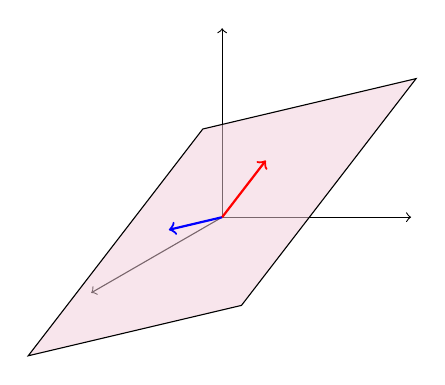
\begin{tikzpicture}[x={(210:0.8cm)}, y={(0:1cm)}, z={(90:1cm)},scale=0.4]
    \draw[->] (0,0,0) -- (6,0,0);
    \draw[->] (0,0,0) -- (0,6,0);
    \draw[->] (0,0,0) -- (0,0,6);
    \draw[fill=purple!20,fill opacity=0.5]
      (-2,-2,2) -- (6,-2,-2) -- (2,2,-2) -- (-6,2,2) -- (-2,-2,2);
    \draw[thick,blue,->] (0,0,0) -- (1,-1,0);
    \draw[thick,red,->] (0,0,0) -- (-2,0,1);
  \end{tikzpicture}
  \end{center}
\end{fact}

\begin{activity}{15}
  Choose any vector \(\begin{bmatrix}\unknown\\\unknown\\\unknown\end{bmatrix}\)
  in \(\IR^3\) that is not in
  \(\vspan\left\{\begin{bmatrix}1\\-1\\0\end{bmatrix},
  \begin{bmatrix}-2\\0\\1\end{bmatrix}\right\}\) by using technology to verify that
  \(
    \RREF
    \begin{bmatrix}[cc|c]1&-2&\unknown\\-1&0&\unknown\\0&1&\unknown\end{bmatrix}
      =
    \begin{bmatrix}[cc|c]1&0&0\\0&1&0\\0&0&1\end{bmatrix}
  \).
  (Why does this work?)
\end{activity}

\begin{fact}
  The set \(\{\vec v_1,\dots,\vec v_m\}\) fails to span all of \(\IR^n\)
  exactly when the vector equation
	\[ x_1 \vec{v}_1 + \cdots x_m\vec{v}_m = \vec{w} \]
  is inconsistent for \textbf{some} vector \(\vec{w}\).
  \vfill
  Note that this happens exactly when \(\RREF[\vec v_1\,\dots\,\vec v_m]\) has a non-pivot row of zeros.
  \[\begin{bmatrix}[cc]1&-2\\-1&0\\0&1\end{bmatrix}\sim
  \begin{bmatrix}[cc]1&0\\0&1\\0&0\end{bmatrix}\]
  \[\Rightarrow
  \begin{bmatrix}[cc|c]1&-2&a\\-1&0&b\\0&1&c\end{bmatrix}\sim
  \begin{bmatrix}[cc|c]1&0&0\\0&1&0\\0&0&1\end{bmatrix}
  \text{for some choice of vector} \begin{bmatrix} a \\ b \\ c \end{bmatrix} \]
\end{fact}

\begin{activity}{5}
  Consider the set of vectors \(S=\left\{
  \begin{bmatrix}2\\3\\0\\-1\end{bmatrix},
  \begin{bmatrix}1\\-4\\3\\0\end{bmatrix},
  \begin{bmatrix}1\\7\\-3\\-1\end{bmatrix},
  \begin{bmatrix}0\\3\\5\\7\end{bmatrix},
  \begin{bmatrix}3\\13\\7\\16\end{bmatrix}
  \right\}
  \).
  Does
  \(\IR^4=\vspan S\)?
	\begin{subactivity}Rewrite this as a question about the solutions to a vector equation.
	\end{subactivity}
	\begin{subactivity}Answer your new question, and use this to answer the original question.
	\end{subactivity}
\end{activity}

\begin{activity}{10}
  Consider the set of third-degree polynomials 
  \begin{align*}
  S=\{
  &2x^3+3x^2-1,
  2x^3+3,
  3x^3+13x^2+7x+16, \\
  &-x^3+10x^2+7x+14,
  4x^3+3x^2+2 \} .
  \end{align*}
  Does
  \(\P^3=\vspan S\)?
	\begin{subactivity}Rewrite this as a question about the solutions to a polynomial equation.
	\end{subactivity}
	\begin{subactivity}Answer your new question, and use this to answer the original question.
	\end{subactivity}
\end{activity}

\begin{activity}{5}
Consider the set of matrices
\[ S = \left\{
		\begin{bmatrix} 1 & 3 \\ 0 & 1 \end{bmatrix},
		\begin{bmatrix} 1 & -1 \\ 1 & 0 \end{bmatrix},
		\begin{bmatrix} 1 & 0 \\ 0 & 2 \end{bmatrix}
		\right\} \]
Does \(M_{2,2} = \vspan S\)?
	\begin{subactivity}Rewrite this as a question about the solutions to a matrix equation.
	\end{subactivity}
	\begin{subactivity}Answer your new question, and use this to answer the original question.
	\end{subactivity}
\end{activity}

\begin{activity}{5}
Let \(\vec{v}_1, \vec{v}_2, \vec{v}_3 \in \IR^7\) be three vectors, and suppose \(\vec{w}\) is another vector with \(\vec{w} \in \vspan \left\{ \vec{v}_1, \vec{v}_2, \vec{v}_3 \right\}\).  What can you conclude about \( \vspan \left\{ \vec{w}, \vec{v}_1, \vec{v}_2, \vec{v}_3 \right\} \) ?
\begin{enumerate}[(a)]
\item \( \vspan \left\{ \vec{w}, \vec{v}_1, \vec{v}_2, \vec{v}_3 \right\} \) is larger than \( \vspan \left\{ \vec{v}_1, \vec{v}_2, \vec{v}_3 \right\} \).
\item \( \vspan \left\{ \vec{w}, \vec{v}_1, \vec{v}_2, \vec{v}_3 \right\}  = \vspan \left\{ \vec{v}_1, \vec{v}_2, \vec{v}_3 \right\} \).
\item \( \vspan \left\{ \vec{w}, \vec{v}_1, \vec{v}_2, \vec{v}_3 \right\} \) is smaller than \( \vspan \left\{ \vec{v}_1, \vec{v}_2, \vec{v}_3 \right\} \).
\end{enumerate}
\end{activity}




\begin{definition}
  A subset of a vector space is called a \term{subspace} if it is
  a vector space on its own.

  \vspace{1em}

  For example, the span of these two vectors forms a planar subspace
  inside of the larger vector space \(\IR^3\).

  \begin{center}
  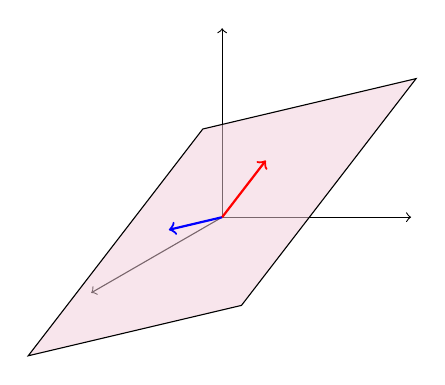
\begin{tikzpicture}[x={(210:0.8cm)}, y={(0:1cm)}, z={(90:1cm)},scale=0.4]
    \draw[->] (0,0,0) -- (6,0,0);
    \draw[->] (0,0,0) -- (0,6,0);
    \draw[->] (0,0,0) -- (0,0,6);
    \draw[fill=purple!20,fill opacity=0.5]
      (-2,-2,2) -- (6,-2,-2) -- (2,2,-2) -- (-6,2,2) -- (-2,-2,2);
    \draw[thick,blue,->] (0,0,0) -- (1,-1,0);
    \draw[thick,red,->] (0,0,0) -- (-2,0,1);
  \end{tikzpicture}
  \end{center}
\end{definition}



\begin{fact}
  Any sub\textbf{set} \(S\) of a vector space \(V\) that contains
  the additive identity \(\vec 0\) satisfies the eight
  vector space properties automatically, since it is a collection of known
  vectors.

  \vspace{1em}

  However, to verify that it's a sub\textbf{space}, we need to check that
  addition and multiplication still make sense using only vectors from \(S\).
  So we need to check two things:

  \begin{itemize}
  \item The set is \term{closed under addition}: for any \(\vec{x},\vec{y} \in S\), the sum \(\vec{x}+\vec{y}\) is also in \(S\).
  \item The set is \term{closed under scalar multiplication}: for any \(\vec{x} \in S\) and scalar \(c \in \IR\), the product \(c\vec{x}\) is also in \(S\).
\end{itemize}
\end{fact}

\begin{activity}{15}
Let \(S=\setBuilder{\begin{bmatrix} x \\ y \\ z \end{bmatrix}}{ x+2y+z=0}\).

\begin{subactivity}
  Let \(\vec{v}=\begin{bmatrix} x \\ y \\ z \end{bmatrix}\) and
  \(\vec{w} = \begin{bmatrix} a \\ b \\ c \end{bmatrix} \) be vectors in \(S\),
  so \(x+2y+z=0\) and \(a+2b+c=0\). Show that
  \(\vec v+\vec w = \begin{bmatrix} x+a \\ y+b \\ z+c \end{bmatrix}\)
  also belongs to \(S\) by verifying that \((x+a)+2(y+b)+(z+c)=0\).
\end{subactivity}
\begin{subactivity}
  Let \(\vec{v}=\begin{bmatrix} x \\ y \\ z \end{bmatrix}\in S\), so
  \(x+2y+z=0\). Show that \(c\vec v=\begin{bmatrix}cx\\cy\\cz\end{bmatrix}\) 
  also belongs to \(S\) for any \(c\in\IR\) by verifying
  an appropriate equation.
\end{subactivity}
\begin{subactivity}
  Is \(S\) is a subspace of \(\IR^3\)?
\end{subactivity}
\end{activity}

\begin{activity}{10}
Let \(S=\setBuilder{\begin{bmatrix} x \\ y \\ z \end{bmatrix}}{ x+2y+z=4}\).
Choose a vector
\(\vec v=\begin{bmatrix} \unknown\\\unknown\\\unknown \end{bmatrix}\) in \(S\)
and a real number \(c=\unknown\), and show that \(c\vec v\) isn't in \(S\).
Is \(S\) a subspace of \(\IR^3\)?
\end{activity}

\begin{remark}
Since \(0\) is a scalar and \(0\vec{v}=\vec{z}\) for any vector \(\vec{v}\), a
nonempty set that is closed under scalar multiplication must contain the zero vector
\(\vec{z}\) for that vector space.

\vspace{1em}

Put another way, you can check any of the following to show that a
nonempty subset \(W\) isn't a subspace:

\begin{itemize}
  \item Show that \(\vec 0\not\in W\). 
  \item Find \(\vec u,\vec v\in W\) such that \(\vec u+\vec v\not\in W\).
  \item Find \(c\in\IR,\vec v\in W\) such that \(c\vec v\not\in W\).
\end{itemize}

If you cannot do any of these, then \(W\) can be proven to be a subspace
by doing the following:
\begin{itemize}
  \item Prove that \(\vec u+\vec v\in W\) whenever \(\vec u,\vec v\in W\).
  \item Prove that \(c\vec v\in W\) whenever \(c\in\IR,\vec v\in W\).
\end{itemize}
\end{remark}

\begin{activity}{20}
  Consider these subsets of \(\IR^3\):
  \[
    R=
    \setBuilder{ \begin{bmatrix}x\\y\\z\end{bmatrix}}{y=z+1}
    \hspace{2em}
    S=
    \setBuilder{ \begin{bmatrix}x\\y\\z\end{bmatrix}}{y=|z|}
    \hspace{2em}
    T=
    \setBuilder{ \begin{bmatrix}x\\y\\z\end{bmatrix}}{z=xy}
  \]
  \begin{subactivity}
  Show \(R\) isn't a subspace by showing that \(\vec 0\not\in R\).
  \end{subactivity}
  \begin{subactivity}
  Show \(S\) isn't a subspace by finding two vectors \(\vec u,\vec v\in S\)
  such that \(\vec u+\vec v\not\in S\).
  \end{subactivity}
  \begin{subactivity}
  Show \(T\) isn't a subspace by finding a vector \(\vec v\in T\)
  such that \(2\vec v\not\in T\).
  \end{subactivity}
\end{activity}



\begin{activity}{5}
Let \(W\) be a subspace of a vector space \(V\).  How are \(\vspan W\) and \(W\) related?
\begin{enumerate}[(a)]
\item \(\vspan W\) is bigger than \(W\)
\item \(\vspan W\) is the same as \(W\)
\item \(\vspan W\) is smaller than \(W\)
\end{enumerate}
\end{activity}

\begin{fact}
  If \(S\) is any subset of a vector space \(V\), then
  since \(\vspan S\) collects all possible linear combinations,
  \(\vspan S\) is automatically a subspace of \(V\).

  \vspace{1em}

  In fact, \(\vspan S\) is always the smallest
  subspace of \(V\) that contains all the vectors in \(S\).
\end{fact}


\begin{activity}{10}
  Consider the two sets
  \begin{align*}
    S=\left\{
  \begin{bmatrix}2\\3\\1\end{bmatrix},
  \begin{bmatrix}1\\1\\4\end{bmatrix}
  \right\} & &
    T=\left\{
  \begin{bmatrix}2\\3\\1\end{bmatrix},
  \begin{bmatrix}1\\1\\4\end{bmatrix},
  \begin{bmatrix}-1\\0\\-11\end{bmatrix}
  \right\}
  \end{align*}
  Which of the following is true?

	\begin{enumerate}[(A)]
	\item \(\vspan S\) is bigger than \(\vspan T\).
	\item \(\vspan S\) and \(\vspan T\) are the same size.
	\item \(\vspan S\) is smaller than \(\vspan T\).
	\end{enumerate}

\end{activity}

\begin{definition}
  We say that a set of vectors is \term{linearly dependent} if one vector
  in the set belongs to the span of the others. Otherwise, we say the set
  is \term{linearly independent}.

  \begin{center}
  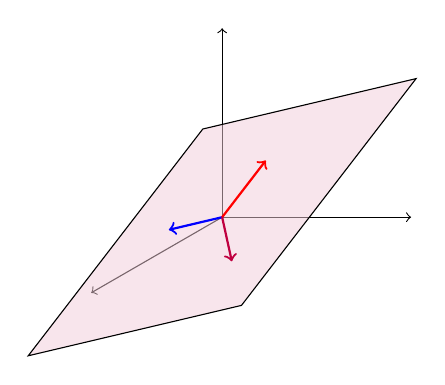
\begin{tikzpicture}[x={(210:0.8cm)}, y={(0:1cm)}, z={(90:1cm)},scale=0.4]
    \draw[->] (0,0,0) -- (6,0,0);
    \draw[->] (0,0,0) -- (0,6,0);
    \draw[->] (0,0,0) -- (0,0,6);
    \draw[fill=purple!20,fill opacity=0.5]
      (-2,-2,2) -- (6,-2,-2) -- (2,2,-2) -- (-6,2,2) -- (-2,-2,2);
    \draw[thick,blue,->] (0,0,0) -- (1,-1,0);
    \draw[thick,red,->] (0,0,0) -- (-2,0,1);
    \draw[thick,purple,->] (0,0,0) -- (1,1,-1);
  \end{tikzpicture}
  \end{center}

  You can think of linearly dependent sets as containing a redundant vector,
  in the sense that you can drop a vector out without reducing the span of the set. In the above image, all three vectors lay on the same planar subspace,
  but only two vectors are needed to span the plane, so the set is
  linearly dependent.
\end{definition}

\begin{activity}{10}
  Let \(\vec{v}_1,\vec{v}_2,\vec{v}_3 \) be vectors in \(\mathbb R^n\).
  Suppose \(3\vec{v}_1-5\vec{v}_2=\vec{v}_3\), so the set
  \(\{\vec{v}_1,\vec{v}_2,\vec{v}_3\}\) is linearly dependent.
  Which of the following is true of the vector equation \(x_1\vec{v}_1+x_2\vec{v}_2+x_3\vec{v}_3=\vec{0}\) ?
  \begin{enumerate}[(A)]
  \item It is consistent with one solution
  \item It is consistent with infinitely many solutions
  \item It is inconsistent.
  \end{enumerate}
\end{activity}

\begin{fact}
  For any vector space,
  the set \(\{\vec v_1,\dots\vec v_n\}\) is linearly dependent if and only
  if the vector equation \(x_1\vec v_1+\dots+x_n\vec v_n=\vec{0}\) is consistent with
  infinitely many solutions.
\end{fact}

\begin{activity}{10}
  Find
  \[\RREF\begin{bmatrix}[ccccc|c]
  2&2&3&-1&4&0\\
  3&0&13&10&3&0\\
  0&0&7&7&0&0\\
  -1&3&16&14&1&0
  \end{bmatrix}
  \]
  and mark the part of the matrix that demonstrates that
  \[S=\left\{
  \begin{bmatrix}2\\3\\0\\-1\end{bmatrix},
  \begin{bmatrix}2\\0\\0\\3\end{bmatrix},
  \begin{bmatrix}3\\13\\7\\16\end{bmatrix},
  \begin{bmatrix}-1\\10\\7\\14\end{bmatrix},
  \begin{bmatrix}4\\3\\0\\1\end{bmatrix}
  \right\}
  \]
  is linearly dependent (the part that shows its linear system has
  infinitely many solutions).
\end{activity}

\begin{quickcheck}
  A set of Euclidean vectors
  \(\{\vec v_1,\dots\vec v_n\}\) is linearly dependent if and only
  if \(\RREF\begin{bmatrix}\vec v_1&\dots&\vec v_n\end{bmatrix}\)
  has a column without a pivot position.
\end{quickcheck}


\begin{observation}
  Compare the following results:
  
  \begin{itemize}
  \item A set of \(\IR^m\) vectors
  \(\{\vec v_1,\dots\vec v_n\}\) is linearly independent if and only
  if \(\RREF\begin{bmatrix}\vec v_1&\dots&\vec v_n\end{bmatrix}\)
  has all pivot columns.
  \item A set of \(\IR^m\) vectors
  \(\{\vec v_1,\dots\vec v_n\}\) spans \(\IR^m\) if and only
  if \(\RREF\begin{bmatrix}\vec v_1&\dots&\vec v_n\end{bmatrix}\)
  has all pivot rows.
  \end{itemize}
\end{observation}

\begin{activity}{5}
  Is the set of Euclidean vectors \(\left\{
  \begin{bmatrix}-4\\2\\3\\0\\-1\end{bmatrix},
  \begin{bmatrix}1\\2\\0\\0\\3\end{bmatrix},
  \begin{bmatrix}1\\10\\10\\2\\6\end{bmatrix},
  \begin{bmatrix}3\\4\\7\\2\\1\end{bmatrix}
  \right\}\) linearly dependent or linearly independent?
\begin{subactivity}
Reinterpret this question as an appropriate question about solutions to a vector equation.
\end{subactivity}
\begin{subactivity} 
Use the solution to this question to answer the original question.
\end{subactivity}
\end{activity}

\begin{activity}{10}
  Is the set of polynomials \(\left\{
  x^3+1,x^2+2x,x^2+7x+4
  \right\}\) linearly dependent or linearly independent?
\begin{subactivity}
Reinterpret this question as an appropriate question about solutions to a polynomial equation.
\end{subactivity}
\begin{subactivity} 
Use the solution to this question to answer the original question.
\end{subactivity}
\end{activity}

\begin{activity}{5}
What is the largest number of \(\IR^4\) vectors that can form a linearly independent set?
\begin{enumerate}[(a)]
\item \(3\)
\item \(4\)
\item \(5\)
\item You can have infinitely many vectors and still be linearly independent.
\end{enumerate}
\end{activity}

\begin{activity}{5}
What is the largest number of 
\[\P^4=\setBuilder{ax^4+bx^3+cx^2+dx+e}{a,b,c,d,e\in\IR}\]
vectors that can form a linearly independent set?
\begin{enumerate}[(a)]
\item \(3\)
\item \(4\)
\item \(5\)
\item You can have infinitely many vectors and still be linearly independent.
\end{enumerate}
\end{activity}

\begin{activity}{5}
What is the largest number of 
\[\P=\setBuilder{f(x)}{f(x)\text{ is any polynomial}}\]
vectors that can form a linearly independent set?
\begin{enumerate}[(a)]
\item \(3\)
\item \(4\)
\item \(5\)
\item You can have infinitely many vectors and still be linearly independent.
\end{enumerate}
\end{activity}






\begin{definition}
  A \term{basis} is a linearly independent set that spans a vector space.

  \vspace{1em}

  The \term{standard basis} of \(\IR^n\) is the set \(\{\vec{e}_1, \ldots, \vec{e}_n\}\) where
  \begin{align*}
  \vec{e}_1 &= \begin{bmatrix}1 \\ 0 \\ 0 \\ \vdots \\ 0 \\  0 \end{bmatrix} &
  \vec{e}_2 &= \begin{bmatrix}0 \\ 1 \\ 0 \\ \vdots \\ 0 \\ 0 \end{bmatrix} &
  \cdots & &
  \vec{e}_n = \begin{bmatrix}0 \\ 0 \\ 0 \\ \vdots \\ 0 \\ 1 \end{bmatrix}
  \end{align*}

  \vspace{1em}

  For \(\IR^3\), these are the vectors
  \(
    \vec e_1=\hat\imath=\begin{bmatrix}1 \\ 0 \\ 0\end{bmatrix},
    \vec e_2=\hat\jmath=\begin{bmatrix}0 \\ 1 \\ 0\end{bmatrix},
  \) and \(
    \vec e_3=\hat k=\begin{bmatrix}0 \\ 0 \\ 1\end{bmatrix}
  \).

  \end{definition}

\begin{observation}
  A basis may be thought of as a collection of building blocks for a vector
  space,  since every vector in the space can be expressed as a unique linear
  combination of basis vectors.

  \vspace{1em}

  For example, in many calculus courses, vectors in \(\IR^3\)
  are often expressed in their component form
  \[
    (3,-2,4)=\begin{bmatrix}3 \\ -2 \\ 4\end{bmatrix}
  \]
  or in their standard basic vector form
  \[
    3\vec e_1-2\vec e_2+4\vec e_3 = 3\hat\imath-2\hat\jmath+4\hat k
  .\]
  Since every vector in \(\IR^3\) can be uniquely described as a linear
  combination of the vectors in \(\setList{\vec e_1,\vec e_2,\vec e_3}\),
  this set is indeed a basis.
\end{observation}



\begin{activity}{15}
  Label each of the sets \(A,B,C,D,E\) as
  \begin{itemize}
     \item SPANS \(\IR^4\) or DOES NOT SPAN \(\IR^4\)
     \item LINEARLY INDEPENDENT or LINEARLY DEPENDENT
     \item BASIS FOR \(\IR^4\) or NOT A BASIS FOR \(\IR^4\)
  \end{itemize}
  by finding \(\RREF\) for their corresponding matrices.
  \begin{center}
    \begin{tabular}{cc}
  	\(A=\left\{
      \begin{bmatrix}1\\0\\0\\0\end{bmatrix},
      \begin{bmatrix}0\\1\\0\\0\end{bmatrix},
      \begin{bmatrix}0\\0\\1\\0\end{bmatrix},
      \begin{bmatrix}0\\0\\0\\1\end{bmatrix}
      \right\}
      \)   &

    \(B=\left\{
      \begin{bmatrix}2\\3\\0\\-1\end{bmatrix},
      \begin{bmatrix}2\\0\\0\\3\end{bmatrix},
      \begin{bmatrix}4\\3\\0\\2\end{bmatrix},
      \begin{bmatrix}-3\\0\\1\\3\end{bmatrix}
      \right\}
      \)  \\


      \(C=\left\{
      \begin{bmatrix}2\\3\\0\\-1\end{bmatrix},
      \begin{bmatrix}2\\0\\0\\3\end{bmatrix},
      \begin{bmatrix}3\\13\\7\\16\end{bmatrix},
      \begin{bmatrix}-1\\10\\7\\14\end{bmatrix},
      \begin{bmatrix}4\\3\\0\\2\end{bmatrix}
      \right\}
      \) &

  	\(D=\left\{
      \begin{bmatrix}2\\3\\0\\-1\end{bmatrix},
      \begin{bmatrix}4\\3\\0\\2\end{bmatrix},
      \begin{bmatrix}-3\\0\\1\\3\end{bmatrix},
      \begin{bmatrix}3\\6\\1\\5\end{bmatrix}
      \right\}
      \) \\

     \(E=\left\{
      \begin{bmatrix}5\\3\\0\\-1\end{bmatrix},
      \begin{bmatrix}-2\\1\\0\\3\end{bmatrix},
      \begin{bmatrix}4\\5\\1\\3\end{bmatrix}
      \right\}
      \)  &
    \end{tabular}
  \end{center}
\end{activity}

\begin{activity}{10}
  If \(\{\vec v_1,\vec v_2,\vec v_3,\vec v_4\}\) is a basis for
  \(\IR^4\), that means \(\RREF[\vec v_1\,\vec v_2\,\vec v_3\,\vec v_4]\)
  doesn't have a non-pivot column, and doesn't have a
  row of zeros. What is \(\RREF[\vec v_1\,\vec v_2\,\vec v_3\,\vec v_4]\)?

  \[
    \RREF[\vec v_1\,\vec v_2\,\vec v_3\,\vec v_4]
      =
    \begin{bmatrix}
      \unknown & \unknown & \unknown & \unknown \\
      \unknown & \unknown & \unknown & \unknown \\
      \unknown & \unknown & \unknown & \unknown \\
      \unknown & \unknown & \unknown & \unknown \\
    \end{bmatrix}
  \]
\end{activity}

\begin{quickcheck}
  The set \(\{\vec v_1,\dots,\vec v_m\}\) is a basis for \(\IR^n\) if and
  only if \(m=n\) and
  \(\RREF[\vec v_1\,\dots\,\vec v_n]=
  \begin{bmatrix}
    1&0&\dots&0\\
    0&1&\dots&0\\
    \vdots&\vdots&\ddots&\vdots\\
    0&0&\dots&1
  \end{bmatrix}
  \).

  That is, a basis for \(\IR^n\) must have exactly \(n\) vectors and
  its square matrix must row-reduce to the so-called \term{identity matrix}
  containing all zeros except for a downward diagonal of ones.
  (We will learn where the identity matrix gets its name in a later module.)
\end{quickcheck}

\begin{observation}
Recall that a \term{subspace} of a vector space is a subset that is itself a vector space.

\vspace{1em}

One easy way to construct a subspace is to take the span of set,
but a linearly dependent set contains ``redundant'' vectors. For example,
only two of the three vectors in the following image are needed to span
the planar subspace.

\begin{center}
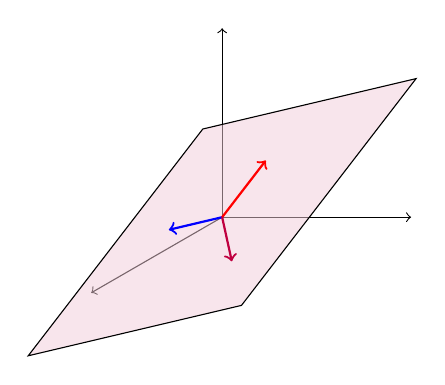
\begin{tikzpicture}[x={(210:0.8cm)}, y={(0:1cm)}, z={(90:1cm)},scale=0.4]
  \draw[->] (0,0,0) -- (6,0,0);
  \draw[->] (0,0,0) -- (0,6,0);
  \draw[->] (0,0,0) -- (0,0,6);
  \draw[fill=purple!20,fill opacity=0.5]
    (-2,-2,2) -- (6,-2,-2) -- (2,2,-2) -- (-6,2,2) -- (-2,-2,2);
  \draw[thick,blue,->] (0,0,0) -- (1,-1,0);
  \draw[thick,red,->] (0,0,0) -- (-2,0,1);
  \draw[thick,purple,->] (0,0,0) -- (1,1,-1);
\end{tikzpicture}
\end{center}
\end{observation}

\begin{activity}{10}
  Consider the subspace of \(\IR^4\) given by \(W=\vspan\left\{
  \begin{bmatrix}2\\3\\0\\1\end{bmatrix},
  \begin{bmatrix}2\\0\\1\\-1\end{bmatrix},
  \begin{bmatrix}2\\-3\\2\\-3\end{bmatrix},
  \begin{bmatrix}1\\5\\-1\\0\end{bmatrix}
  \right\}
  \).

  \begin{subactivity}
    Mark the part of \(\RREF\begin{bmatrix}
    2&2&2&1\\
    3&0&-3&5\\
    0&1&2&-1\\
    1&-1&-3&0
    \end{bmatrix}\) that shows that \(W\)'s spanning set
    is linearly dependent.
  \end{subactivity}

  \begin{subactivity}
    Find a basis for \(W\) by removing a vector from its spanning set
    to make it linearly independent.
  \end{subactivity}
\end{activity}

\begin{fact}
  Let \(S=\{\vec v_1,\dots,\vec v_m\}\). The easiest basis describing
  \(\vspan S\) is the set of vectors in \(S\) given by the pivot columns
  of \(\RREF[\vec v_1\,\dots\,\vec v_m]\).

  \vspace{1em}

  Put another way, to compute a basis for the subspace \(\vspan S\),
  simply remove the vectors corresponding to the non-pivot columns of
  \(\RREF[\vec v_1\,\dots\,\vec v_m]\).
  For example, since
  \[
    \RREF
    \begin{bmatrix}
      1 & 2 & 3 \\
      0 & -2 & -2 \\
      -3 & 1 & -2
    \end{bmatrix}
      =
    \begin{bmatrix}
      \circledNumber{1} & 0 & 1 \\
      0 & \circledNumber{1} & 1 \\
      0 & 0 & 0
    \end{bmatrix}
  \]
  the subspace
  \(
    W=\vspan\setList{
      \begin{bmatrix}1\\0\\-3\end{bmatrix},
      \begin{bmatrix}2\\-2\\1\end{bmatrix},
      \begin{bmatrix}3\\-2\\-2\end{bmatrix}
    }
  \)
  has
  \(
    \setList{
      \begin{bmatrix}1\\0\\-3\end{bmatrix},
      \begin{bmatrix}2\\-2\\1\end{bmatrix}
    }
  \)
  as a basis.
\end{fact}

\begin{activity}{10}
Let \(W\) be the subspace of \(\IR^4\) given by
 \[W = \vspan \left\{
 \begin{bmatrix} 1 \\ 3 \\ 1 \\ -1 \end{bmatrix},
 \begin{bmatrix} 2 \\ -1 \\ 1 \\ 2 \end{bmatrix},
 \begin{bmatrix} 4 \\ 5 \\ 3 \\ 0 \end{bmatrix},
 \begin{bmatrix} 3 \\ 2 \\ 2 \\ 1 \end{bmatrix}
 \right\}. \]
 Find a basis for \(W\).
\end{activity}

\begin{activity}{10}
Let \(W\) be the subspace of \(\P^3\) given by
 \[W = \vspan \left\{x^3+3x^2+x-1, 2x^3-x^2+x+2, 4x^3+5x^2+3x, 3x^3+2x^2+2x+1 \right\} \]
 Find a basis for \(W\).
\end{activity}

\begin{activity}{10}
Let \(W\) be the subspace of \(M_{2,2}\) given by
 \[W = \vspan \left\{
 \begin{bmatrix} 1 & 3 \\ 1  & -1 \end{bmatrix},
 \begin{bmatrix} 2 & -1 \\ 1  & 2 \end{bmatrix},
 \begin{bmatrix} 4 & 5 \\ 3  & 0 \end{bmatrix},
 \begin{bmatrix} 3 & 2 \\ 2  & 1 \end{bmatrix}
 \right\}. \]
 Find a basis for \(W\).
\end{activity}

\begin{observation}
  In the previous section, we learned that
  computing a basis for the subspace \(\vspan\{\vec v_1,\dots,\vec v_m\}\),
  is as simple as removing the vectors corresponding to the non-pivot columns of
  \(\RREF[\vec v_1\,\dots\,\vec v_m]\).

  \vspace{1em}

  For example, since
  \[
    \RREF
    \begin{bmatrix}
      1 & 2 & 3 \\
      0 & -2 & -2 \\
      -3 & 1 & -2
    \end{bmatrix}
      =
    \begin{bmatrix}
      \circledNumber{1} & 0 & 1 \\
      0 & \circledNumber{1} & 1 \\
      0 & 0 & 0
    \end{bmatrix}
  \]
  the subspace
  \(
    W=\vspan\setList{
      \begin{bmatrix}1\\0\\-3\end{bmatrix},
      \begin{bmatrix}2\\-2\\1\end{bmatrix},
      \begin{bmatrix}3\\-2\\-2\end{bmatrix}
    }
  \)
  has
  \(
    \setList{
      \begin{bmatrix}1\\0\\-3\end{bmatrix},
      \begin{bmatrix}2\\-2\\1\end{bmatrix}
    }
  \)
  as a basis.
\end{observation}

\begin{activity}{10}
  Let
  \begin{align*}
  S=\left\{
  \begin{bmatrix}2\\3\\0\\1\end{bmatrix},
  \begin{bmatrix}2\\0\\1\\-1\end{bmatrix},
  \begin{bmatrix}2\\-3\\2\\-3\end{bmatrix},
  \begin{bmatrix}1\\5\\-1\\0\end{bmatrix}
  \right\} & & \text{and}  & &
  T=\left\{
  \begin{bmatrix}2\\0\\1\\-1\end{bmatrix},
  \begin{bmatrix}2\\-3\\2\\-3\end{bmatrix},
  \begin{bmatrix}1\\5\\-1\\0\end{bmatrix},
  \begin{bmatrix}2\\3\\0\\1\end{bmatrix}
  \right\}
  \end{align*}
  \begin{subactivity}
  Find a basis for \(\vspan S\).
  \end{subactivity}
  \begin{subactivity}
  Find a basis for \(\vspan T\).
  \end{subactivity}
\end{activity}

\begin{observation}
  Even though we found different bases for them,
  \(\vspan S\) and \(\vspan T\) are exactly the same subspace of \(\IR^4\),
  since
  \[
    S=\left\{
    \begin{bmatrix}2\\3\\0\\1\end{bmatrix},
    \begin{bmatrix}2\\0\\1\\-1\end{bmatrix},
    \begin{bmatrix}2\\-3\\2\\-3\end{bmatrix},
    \begin{bmatrix}1\\5\\-1\\0\end{bmatrix}
    \right\}
      =
    \left\{
    \begin{bmatrix}2\\0\\1\\-1\end{bmatrix},
    \begin{bmatrix}2\\-3\\2\\-3\end{bmatrix},
    \begin{bmatrix}1\\5\\-1\\0\end{bmatrix},
    \begin{bmatrix}2\\3\\0\\1\end{bmatrix}
    \right\}=T
  \]
\end{observation}


\begin{fact}
  Any non-trivial vector space has infinitely-many different bases, but all
  the bases for a given vector space are exactly the same size.

  \vspace{1em}

  For example,
  \[
    \setList{\vec e_1,\vec e_2,\vec e_3}
      \text{ and }
    \setList{
      \begin{bmatrix}1\\0\\0\end{bmatrix},
      \begin{bmatrix}0\\1\\0\end{bmatrix},
      \begin{bmatrix}1\\1\\1\end{bmatrix}
    }
      \text{ and }
    \setList{
      \begin{bmatrix}1\\0\\-3\end{bmatrix},
      \begin{bmatrix}2\\-2\\1\end{bmatrix},
      \begin{bmatrix}3\\-2\\5\end{bmatrix}
    }
  \]
  are all valid bases for \(\IR^3\), and they all contain three vectors.
\end{fact}

\begin{definition}
  The \term{dimension} of a vector space is equal to the size
  of any basis for the vector space.

  \vspace{1em}

  As you'd expect, \(\IR^n\) has dimension \(n\).
  For example, \(\IR^3\) has dimension \(3\) because any basis for \(\IR^3\)
  such as
  \[
    \setList{\vec e_1,\vec e_2,\vec e_3}
      \text{ and }
    \setList{
      \begin{bmatrix}1\\0\\0\end{bmatrix},
      \begin{bmatrix}0\\1\\0\end{bmatrix},
      \begin{bmatrix}1\\1\\1\end{bmatrix}
    }
      \text{ and }
    \setList{
      \begin{bmatrix}1\\0\\-3\end{bmatrix},
      \begin{bmatrix}2\\-2\\1\end{bmatrix},
      \begin{bmatrix}3\\-2\\5\end{bmatrix}
    }
  \]
  contains exactly three vectors.
\end{definition}

\begin{activity}{10}
  Find the dimension of each subspace of \(\IR^4\) by finding
  \(\RREF\) for each corresponding matrix.

  \begin{center}
	\begin{tabular}{ll}

     \(\vspan\left\{
    \begin{bmatrix}2\\3\\0\\-1\end{bmatrix},
    \begin{bmatrix}2\\0\\0\\3\end{bmatrix},
    \begin{bmatrix}4\\3\\0\\2\end{bmatrix},
    \begin{bmatrix}-3\\0\\1\\3\end{bmatrix}
    \right\}
    \)

 &
     \(\vspan\left\{
    \begin{bmatrix}2\\3\\0\\-1\end{bmatrix},
    \begin{bmatrix}2\\0\\0\\3\end{bmatrix},
    \begin{bmatrix}3\\13\\7\\16\end{bmatrix},
    \begin{bmatrix}-1\\10\\7\\14\end{bmatrix},
    \begin{bmatrix}4\\3\\0\\2\end{bmatrix}
    \right\}
    \)
 \\
     \(\vspan\left\{
    \begin{bmatrix}2\\3\\0\\-1\end{bmatrix},
    \begin{bmatrix}4\\3\\0\\2\end{bmatrix},
    \begin{bmatrix}-3\\0\\1\\3\end{bmatrix},
    \begin{bmatrix}3\\6\\1\\5\end{bmatrix}
    \right\}
    \)

 &
     \(\vspan\left\{
    \begin{bmatrix}5\\3\\0\\-1\end{bmatrix},
    \begin{bmatrix}-2\\1\\0\\3\end{bmatrix},
    \begin{bmatrix}4\\5\\1\\3\end{bmatrix}
    \right\}
	\)
\end{tabular}
\end{center}
\end{activity}

\begin{fact}
  Every vector space with finite dimension, that is, every
  vector space \(V\) with a basis of the form
  \(\{\vec v_1,\vec v_2,\dots,\vec v_n\}\) is said to be
  \term{isomorphic} to a Euclidean space \(\IR^n\), since there exists
  a natural correspondance between vectors in \(V\) and vectors in \(\IR^n\):

  \[
    c_1\vec v_1+c_2\vec v_2+\dots+c_n\vec v_n
    \leftrightarrow
    \begin{bmatrix}
      c_1\\c_2\\\vdots\\c_n
    \end{bmatrix}
  \]
\end{fact}

\begin{observation}
  We've already been taking advantage of the previous fact by converting
  polynomials and matrices into Euclidean vectors. Since \(\P^3\)
  and \(M_{2,2}\) are both four-dimensional:

  \[
    4x^3+0x^2-1x+5
    \leftrightarrow
    \begin{bmatrix}
      4\\0\\-1\\5
    \end{bmatrix}
    \leftrightarrow
    \begin{bmatrix}
      4&0\\-1&5
    \end{bmatrix}
  \]
\end{observation}

\begin{activity}{5}
Suppose \(W\) is a subspace of \(\P^8\), and you know that
 the set \(\{ x^3+x, x^2+1, x^4-x \}\) is a linearly independent subset of \(W\).
What can you conclude about \(W\)?
\begin{enumerate}[(a)]
\item The dimension of \(W\) is at most 3.
\item The dimension of \(W\) is exactly 3.
\item The dimension of \(W\) is at least 3.
\end{enumerate}
\end{activity}

\begin{activity}{5}
Suppose \(W\) is a subspace of \(\P^8\), and you know that
 \(W\) is spanned by the six vectors \[\{ x^4-x,x^3+x,x^3+x+1,x^4+2x,x^3,2x+1\}.\]
What can you conclude about \(W\)?
\begin{enumerate}[(a)]
\item The dimension of \(W\) is at most 6.
\item The dimension of \(W\) is exactly 6.
\item The dimension of \(W\) is at least 6.
\end{enumerate}
\end{activity}

\begin{observation}
  The space of polynomials \(\P\) (of \textit{any} degree)
  has the basis \(\{1,x,x^2,x^3,\dots\}\),
  so it is a natural example of an infinite-dimensional vector space.

  \vspace{1em}

  Since \(\P\) and other infinite-dimensional spaces cannot be treated as
  an isomorphic finite-dimensional Euclidean space \(\IR^n\), vectors in
  such spaces cannot be studied by converting them into Euclidean vectors.
  Fortunately, most of the examples we will be
  interested in for this course will be finite-dimensional.
\end{observation}

\begin{definition}
A \term{homogeneous} system of linear equations is one of the form:
  \begin{alignat*}{5}
    a_{11}x_1 &\,+\,& a_{12}x_2 &\,+\,& \dots  &\,+\,& a_{1n}x_n &\,=\,& 0 \\
    a_{21}x_1 &\,+\,& a_{22}x_2 &\,+\,& \dots  &\,+\,& a_{2n}x_n &\,=\,& 0 \\
     \vdots&  &\vdots&   &&  &\vdots&&\vdots  \\
    a_{m1}x_1 &\,+\,& a_{m2}x_2 &\,+\,& \dots  &\,+\,& a_{mn}x_n &\,=\,& 0
  \end{alignat*}

  This system is equivalent to the vector equation:
  \[x_1 \vec{v}_1 + \cdots+x_n \vec{v}_n = \vec{0}\]
  and the augmented matrix:
  \[
    \begin{bmatrix}[cccc|c]
      a_{11} & a_{12} & \cdots & a_{1n} & 0\\
      a_{21} & a_{22} & \cdots & a_{2n} & 0\\
      \vdots & \vdots & \ddots & \vdots & \vdots\\
      a_{m1} & a_{m2} & \cdots & a_{mn} & 0
    \end{bmatrix}
  \]
\end{definition}

\begin{activity}{5}
Note that if \(\begin{bmatrix} a_1 \\ \vdots \\ a_n \end{bmatrix} \) and
\(\begin{bmatrix} b_1 \\ \vdots \\ b_n \end{bmatrix} \) are solutions to
\(x_1 \vec{v}_1 + \cdots+x_n \vec{v}_n = \vec{0}\)
so is  \(\begin{bmatrix} a_1 +b_1\\ \vdots \\ a_n+b_n \end{bmatrix} \), since
\[a_1 \vec{v}_1+\cdots+a_n \vec{v}_n = \vec{0}
\text{ and }
b_1 \vec{v}_1+\cdots+b_n \vec{v}_n = \vec{0} \]
implies
\[(a_1 + b_1) \vec{v}_1+\cdots+(a_n+b_n) \vec{v}_n = \vec{0} .\]

Similarly, if \(c \in \IR\), \(\begin{bmatrix} ca_1 \\ \vdots \\ ca_n \end{bmatrix} \) is a solution.
Thus the solution set of a homogeneous system is...
\begin{multicols}{3}
\begin{enumerate}[a)]
  \item A basis for \(\IR^n\).
  \item A subspace of \(\IR^n\).
  \item The empty set.
\end{enumerate}
\end{multicols}
\end{activity}

\begin{activity}{10}
Consider the homogeneous system of equations
\begin{alignat*}{5}
x_1&\,+\,&2x_2&\,\,& &\,+\,& x_4 &=& 0 \\
2x_1&\,+\,&4x_2&\,-\,&x_3 &\,-\,&2 x_4 &=& 0 \\
3x_1&\,+\,&6x_2&\,-\,&x_3 &\,-\,& x_4 &=& 0 \\
\end{alignat*}
\begin{subactivity}
Find its solution set (a subspace of \(\IR^4\)).
\end{subactivity}
\begin{subactivity}
Rewrite this solution space in the form \[\setBuilder{ a \begin{bmatrix} \unknown \\ \unknown \\ \unknown \\ \unknown\end{bmatrix} + b \begin{bmatrix} \unknown \\ \unknown \\ \unknown \\ \unknown \end{bmatrix} }{a,b \in \IR}.\]
\end{subactivity}
\begin{subactivity}
Rewrite this solution space in the form \[\vspan\left\{\begin{bmatrix} \unknown \\ \unknown \\ \unknown \\ \unknown\end{bmatrix}, \begin{bmatrix} \unknown \\ \unknown \\ \unknown \\ \unknown \end{bmatrix}\right\}.\]
\end{subactivity}
\end{activity}

\begin{fact}
  The coefficients of the free variables in the solution set of a linear system
  always yield linearly independent vectors.

  \vspace{1em}

  Thus if
  \[
    \setBuilder{
      a \begin{bmatrix} -2 \\ 1 \\ 0 \\ 0\end{bmatrix} +
      b \begin{bmatrix} -1 \\ 0 \\ -4 \\ 1 \end{bmatrix}
    }{
      a,b \in \IR
    } = \vspan\left\{ \begin{bmatrix} -2 \\ 1 \\ 0 \\ 0\end{bmatrix}, 
					 \begin{bmatrix} -1 \\ 0 \\ -4 \\ 1 \end{bmatrix} \right\}
  \]
  is the solution space for a homogeneous system, then
  \[
    \setList{
      \begin{bmatrix} -2 \\ 1 \\ 0 \\ 0\end{bmatrix},
      \begin{bmatrix} -1 \\ 0 \\ -4 \\ 1 \end{bmatrix}
    }
  \]
  is a basis for the solution space.
\end{fact}



\begin{activity}{10}
Consider the homogeneous system of equations
\begin{alignat*}{5}
2x_1&\,+\,&4x_2&\,+\,& 2x_3&\,-\,&4x_4  &=& 0 \\
-2x_1&\,-\,&4x_2&\,+\,&x_3 &\,+\,& x_4 &=& 0 \\
3x_1&\,+\,&6x_2&\,-\,&x_3 &\,-\,&4 x_4 &=& 0 \\
\end{alignat*}

Find a basis for its solution space.
\end{activity}

\begin{activity}{10}
Consider the homogeneous vector equation
\[ 
   x_1 \begin{bmatrix} 2 \\ -2 \\ 3 \end{bmatrix}+
   x_2 \begin{bmatrix} 4 \\ -4 \\ 6 \end{bmatrix}+
   x_3 \begin{bmatrix} 2 \\ 1 \\ -1 \end{bmatrix}+
   x_4 \begin{bmatrix} -4 \\ 1 \\ -4 \end{bmatrix}=
       \begin{bmatrix} 0 \\ 0 \\ 0 \end{bmatrix}
\]


Find a basis for its solution space.
\end{activity}

\begin{activity}{5}
Consider the homogeneous system of equations
\begin{alignat*}{5}
x_1&\,-\,&3x_2&\,+\,& 2x_3  &=& 0 \\
2x_1&\,+\,&6x_2&\,+\,&4x_3  &=& 0 \\
x_1&\,+\,&6x_2&\,-\,&4x_3 &=& 0 \\
\end{alignat*}

Find a basis for its solution space.
\end{activity}

\begin{observation}
The basis of the trivial vector space is the empty set.  You can denote this as either \(\emptyset\) or \(\{\}\).
\vfill
Thus, if \(\vec{0}\) is the only solution of a homogeneous system, the basis of the solution space is  \(\emptyset\).
\end{observation}

